% !TeX encoding = UTF-8
% !TeX spellcheck = en_US

\chapter{Graph Transformation Java API}
\label{api}
This chapter describes how a typed Java API can be extracted from the textual specification such that the specified patterns and rules can be invoked from Java code without casting all results and losing type safety (Section~\ref{api-code-generation}).
Section~\ref{gt-interpreter} describes how the API delegates method calls to the graph transformation interpreter, while Section~\ref{api-usage} deals with the usage of the API.
Finally, Section~\ref{incrementality} presents the realization of features which exploit the incrementality of the underlying pattern matcher.

\section{Code Generation for a Typed Java API}
\label{api-code-generation}
The graph transformation specification is placed in a graph transformation project in the Eclipse IDE.\footnote{Any Java and plugin project will be automatically converted to a graph transformation project when adding at least one \texttt{gt} file via the wizard.
	Note that Eclipse projects can have multiple natures: A graph transformation project must have at least the GT, Java and plugin nature.}
All \texttt{gt} files must be placed in the \texttt{src} folder of the project.
For each package containing at least one \texttt{gt} file an API will be generated.
The generated code and models will be placed in corresponding packages in the \texttt{src-gen} folder.

Figure~\ref{fig:api-classes} gives an overview of the API classes assuming there is a package \texttt{example} containing a \texttt{gt} file with a pattern \texttt{ex1()} and a rule \texttt{ex2()}.
For clarity, the class diagram shows only a small subset of the methods implemented by the abstract super classes.
The API serves as a factory for patterns and rules as it provides methods for all non-abstract patterns and rules defined in the package.
The app provides utility methods to create or load EMF resources and add them to the model and initialize the API for a concrete pattern matching engine.
Within the packages \texttt{example.api.rules} and \texttt{example.api.matches} subclasses for the concrete patterns and rules are generated:
\begin{itemize}
	\item The pattern/rule class contains methods for binding context and deleted nodes (except local ones) to a specific object (cp. Section~\ref{api-node-bindings} for more information on node binding).
	If a pattern/rule has parameters (cp. Section~\ref{api-parameters}), they must be initialized in the constructor.
	In addition, setters for all parameters are generated.
	\item The match class contains getters for all nodes in the pattern/rule except the ones marked as local.
\end{itemize}

\noindent
Pattern and rule classes inherit from a super class, \texttt{GraphTransformationPattern} or \texttt{GraphTransformationRule}.
Match classes inherit from \texttt{GraphTransformationMatch}.
These super classes are abstract and implement all methods which are independent from a concrete specification such that only a minimal subset of method implementation needs to be generated.

\begin{figure}[H]
	\centering
	\begin{adjustwidth}{-15mm}{}
		% !TeX encoding = UTF-8
% !TeX spellcheck = en_US

\begin{tikzpicture}
	\begin{umlpackage}[x = 0, y = 0, name=api]{org.emoflon.ibex.gt.api}
		\umlabstract[class, x = 0.8, y = 0]
			{GraphTransformationApp}{
				\# resourceSet: ResourceSet
			}{
				\umlvirt{\# registerMetaModels()} \methodSep
				\umlvirt{\# initAPI(): API}
			}

		\umlabstract[class, x = 0.8, y = -3]
			{GraphTransformationAPI}{}{
				+ getModel(): ResourceSet \methodSep
				+ setDPO() \methodSep
				+ setSPO() \methodSep
				+ updateMatches()
			}

		\umlabstract[class, x = 0.8, y = -7.7]
			{GraphTransformationPattern}{
				\# parameters: Map$<$String, Object$>$
			}{
				\umlvirt{\# convertMatch(IMatch): M} \methodSep
				+ findAnyMatch(): Optional$<$M$>$ \methodSep
				+ findMatches(): Collection$<$M$>$ \methodSep
				+ getParameters(): Map$<$String, Object$>$ \methodSep
				\umlvirt{\# getParameterNames(): List$<$String$>$} \methodSep
				+ subscribeAppearing(Consumer$<$M$>$) \methodSep
				+ subscribeDisappearing(Consumer$<$M$>$) \methodSep
				+ subscribeMatchDisappears(M, Consumer$<$M$>$)
			}

		\umlabstract[class, x = 1.2, y = -12.2]
			{GraphTransformationRule}{}{
				+ apply(): Optional$<$M$>$ \methodSep
				+ setDPO() \methodSep
				+ setSPO()
			}

		\umlabstract[class, x = 1.2, y = -14]
			{GraphTransformationMatch}{}{}
	\end{umlpackage}
	
	\umlinherit
		{GraphTransformationRule}
		{GraphTransformationPattern}
	\umluniassoc[arg2=api, pos2= 0.5]
		{GraphTransformationPattern}
		{GraphTransformationAPI}
	\umluniassoc[arg2=pattern, pos2 = 1.6, align2=right, anchor2 = -132, geometry=-|]
		{GraphTransformationMatch}
		{GraphTransformationPattern}

	\begin{umlpackage}[x = 3.5, y = -17.3, name=engine]{org.emoflon.ibex.gt.engine}
		\umlclass[class, x = 0, y = 0]
			{GraphTransformationInterpreter}{}{
				+ apply(IMatch, PushoutApproach, Map$<$String, Object$>$): Optional$<$IMatch$>$ \methodSep
				+ matchStream(String, Map$<$String, Object$>$): Stream$<$IMatch$>$
			}
	\end{umlpackage}

	\umluniassoc[arg2=interpreter, pos2 = 2, geometry=-|-, arm1=-4.5cm]
		{GraphTransformationAPI}
		{GraphTransformationInterpreter}
	\umluniassoc[geometry=-|-, arm1=-4.5cm]
		{GraphTransformationPattern}
		{GraphTransformationInterpreter}

	\begin{umlpackage}[x = 7.7, y = 0, name = exampleapi]{example.api}
		\umlclass[class, x = 0, y = 0]
			{ExampleApp}{}{}

		\umlclass[class, x = 0, y = -1.8]
			{ExampleAPI}{}{
				+ ex1(): Ex1Pattern \methodSep
				+ ex2(): Ex2Rule
			}
	\end{umlpackage}

	\umlinherit
		{ExampleApp}
		{GraphTransformationApp}
	\umlinherit[geometry=-|-, arm1 = -2.3cm]
		{ExampleAPI}
		{GraphTransformationAPI}

	\begin{umlpackage}[x = 8, y = -5.5, name = exampleapirules]{example.api.rules}
		\umlclass[class, x = 0, y = 0]
			{Ex1Pattern}{}{
				+ bindA(A): Ex1Pattern
			}

		\umlclass[class, x = 0, y = -1.8]
			{Ex2Rule}{}{
				+ bindA(A): Ex2Rule
			}
	\end{umlpackage}

	\umlinherit[geometry=-|-, arm1 = -2.6cm, anchor2 = 20]
		{Ex1Pattern}
		{GraphTransformationPattern}
	\umlinherit[geometry=-|-, arm1 = -2.6cm]
		{Ex2Rule}
		{GraphTransformationRule}

	\begin{umlpackage}[x = 7.05, y = -11, name = exampleapimatches]{example.api.matches}
		\umlclass[class, x = 0, y = 0]
			{Ex1Match}{}{
				+ getA(): A
			}

		\umlclass[class, x = 2.5, y = 0]
			{Ex2Match}{}{
				+ getA(): A \methodSep
				+ getB(): B
			}
	\end{umlpackage}

	\umlinherit[geometry=|-, arm1 = -2.5cm]
		{Ex1Match}
		{GraphTransformationMatch}
	\umlinherit[geometry=|-, arm1 = -2.5cm]
		{Ex2Match}
		{GraphTransformationMatch}
\end{tikzpicture}

	\end{adjustwidth}
	\caption{Overview of the API Java Classes}
	\label{fig:api-classes}
\end{figure}

\noindent
One difference to other graph transformation tools which provide an API for the specified rules (\eg EMorF, Henshin)\footnote{The tool Viatra \cite{VIATRAWebsite} also provides a generated, typed API in a similar way as eMoflon::IBeX-GT, but cannot handle rule applications.} is that the API generated by eMoflon::IBeX-GT is typed to avoid casting in the code using the API (cp. Section~\ref{api-usage}).
If the usage of the API does not fit to the pattern or rule specification, the developer will get error messages at compile time instead of class cast exceptions at runtime.
The typing in the API requires generated code for the meta-models used in the patterns and rules, as the interfaces of those are referenced in the generated API code.
Per default, eMoflon::IBeX-GT assumes that the generated code for the meta-model is in a Java package named as the package in the Ecore file of the meta-model.
This can be adjusted for custom use cases via a setting in a properties file.\footnote{see appendix of the handbook \cite{eMoflonIBeX-GT-Handbook}, Section ``Frequently Asked Questions''}

\section{Graph Transformation Interpreter}
\label{gt-interpreter}
The interaction of the \texttt{GraphTransformationInterpreter} and the API is explained in this section.
The interpreter is independent of a concrete rule specification and ignores typing (\ie everything is an \texttt{Object} in the method signatures, cp. Figure~\ref{fig:api-classes}).
The API provides a typed interface for the graph transformation interpreter such that all methods only accept objects of the correct type as defined in the editor specification.
Figure~\ref{fig:api-and-interpreter} illustrates how the API classes (shown with a purple border) use the graph transformation interpreter (olive border).
The interpreters for context, deletion and creation are shown in their typical colors black, red and green.

\begin{figure}[h!]
	\centering
	% !TeX encoding = UTF-8
% !TeX spellcheck = en_US

\begin{tikzpicture} [
		auto,
		node distance = 4cm,
		node/.style = {
			rectangle,
			rounded corners,
			thick,
			text width = 6em,
			text centered,
			minimum height = 3em
		},
		api/.style = {
			node,
			text width = 5em,
			draw = purple
		},
		gt-interpreter/.style = {
			node,
			text width = 8em,
			draw = olive
		},
		edge/.style = {
			->,
			thick
		}
	]

	\node[api] (api) {
		...API
	};
	\node[api, below of = api] (pattern) {
		...Pattern \\
		or ...Rule
	};
	\node[api, below of = pattern] (match) {
		...Match
	};

	\node[gt-interpreter, right = 2.2cm of pattern] (interpreter) {
		graph transformation interpreter
	};

	\node[node, draw = red, right = 2cm of interpreter] (delete-interpreter) {
		delete interpreter
	};
	\node[node, draw = black, above of = delete-interpreter] (context-interpreter) {
		pattern matcher
	};
	\node[node, draw = green, below of = delete-interpreter] (create-interpreter) {
		create interpreter
	};

	\draw[edge] (api) -- node[left] {creates instances} (pattern);
	\draw[edge] (pattern) -- node[left] {converts matches} (match);

	\draw[edge] (pattern.60) -- ++(0,1.5) -- ++(4.55,0) node[above, pos = 0.5] {fetch matches}  -- (interpreter.100);
	\draw[edge] (interpreter.130) -- ++(0,0.5) -- ++(-3.8,0) node[above, pos = 0.5] {filters \& returns matches} -- (pattern.40);
	
	\draw[edge] (pattern.300) -- ++(0,-1.5) -- ++(4.55,0) node[below, pos = 0.5] {subscribe matches} -- (interpreter.260);
	\draw[edge] (interpreter.230) -- ++(0,-0.5) -- ++(-3.8,0) node[below, pos = 0.5] {notify of matches} -- (pattern.320);
	
	\draw[edge] (interpreter.40) -- ++(0,3.5) -- node[] {initializes} (context-interpreter.175);
	\draw[edge] (context-interpreter.185) -- node[yshift = 0.2cm] {reports matches} (interpreter.30);
	\draw[edge] (interpreter) -- node[text width = 1.5cm] {delegates deletion} (delete-interpreter);
	\draw[edge] (interpreter) -- node[xshift = -0.2cm] {delegates creation} (create-interpreter.west);
\end{tikzpicture}

	\caption{API and Graph Transformation Interpreter}
	\label{fig:api-and-interpreter}
\end{figure}

\noindent
The graph transformation interpreter initializes the pattern matching engine (Democles) by registering the pattern set.
Democles will report any appearing and disappearing matches such that the graph transformation interpreter can maintain a set of \texttt{IMatch}es for each pattern.
\texttt{IMatch}es are an untyped representation of matches, which abstracts from the structure in the concrete pattern matching engine.

Remember that the API class is a factory for patterns and rules, \ie the methods return an instance of a pattern or a rule.
On a pattern/rule instance nodes and parameters can be bound to a fixed value (cp. the following section for details).
When a method for querying matches is called on a pattern or a rule, the call is delegated to the graph transformation interpreter which will return the matches as a \texttt{Stream} of \texttt{IMatch}es.
Using a \texttt{Stream}, unnecessary conversions between \texttt{Stream}s and collections can be avoided in the implementation of the API.
If nodes are bound or parameters are set, the matches will be filtered according to the fixed nodes or parameter values.
If a pattern is defined as being one of multiple alternative patterns, the graph transformation interpreter will combine the matches of all alternative patterns and remove duplicates (cp. Section~\ref{disjunctions}).
Before a pattern or a rule returns the matches, these matches are converted to a typed representation.

Before a rule can be applied, a match must be found where the rule can be applied to.
If a rule contains only created elements, the rule is always applicable. An empty match will be generated in this special case.
Rule applications are delegated to the delete and the create interpreter which handle the rule application according to the defined pushout approach using the create or delete patterns from the IBeX model.

\section{Usage of the API}
\label{api-usage}
This section deals with the usage of the Java API.
The API features are explained using small example code snippets.

\subsection{Initialization and Conventions on EMF Resources}
\label{api-conventions}
An EMF model is assumed to be represented by a \texttt{ResourceSet}, containing one or more resources (files, usually having the file extension \texttt{xmi}).
If not explicitly specified, the first resource in the \texttt{ResourceSet} is chosen as default resource.
All created nodes whose resource is not determined automatically due to their container object, will be placed in the default resource.
Deleted nodes will be moved to a trash resource, which is created automatically.

The generated app class provides convenient methods for model initialization and setting the default resource.
The meta-models used by the patterns and rules in the API will be registered automatically.
The easiest way to initialize an API with a model is to implement a subclass of the Democles app generated in the API package, as shown in Listing~\ref{listing:loading-models}.
As the method names suggest, the method \texttt{createModel(URI)} creates a new empty resource with the given URI, while \texttt{loadModel(URI)} loads an existing resource.

In this case, the file \texttt{newModel.xmi} will be the default resource such that created elements will be added to this file -- except if the container of the created elements is an object in the file \texttt{model.xmi}.
To use \texttt{model.xmi} as the default resource, it can be set via \texttt{setDefaultResource(Resource)}. Alternatively, changing the order of the two method calls adding a resource to the model will lead to the same result.

\begin{lstlisting}[caption={Loading Models}, label={listing:loading-models}]
public class MyGTApp extends SheRememberedCaterpillarsGraphTransformationDemoclesApp {
	SheRememberedCaterpillarsGraphTransformationAPI api;

	public MyGTApp() {
		String path = "./instances/";
		createModel(URI.createFileURI(path + "newModel.xmi"));
		loadModel(URI.createFileURI(path + "model.xmi"));

		api = initAPI();
	}

	public static void main(String[] args) {
		new MyGTApp();
	}
}
\end{lstlisting}

\subsection{Model Queries}
\label{api-model-queries}
Listing~\ref{listing:model-queries} shows examples how the model can be queried via the API using the pattern \texttt{findCharacterOnExit} (Figure~\ref{fig:pattern-findCharacterOnExit}).
All methods for querying matches fetch the untyped matches from the interpreter and convert the matches into the typed representation.
To get the number of matches, one should always use the method \texttt{countMatches()} because the implementation avoids the conversion.

\begin{lstlisting}[caption={Model Queries}, label={listing:model-queries}]
public Optional<Character> findAnyCharacter() {
	return api.findCharacterOnExit()
		.findAnyMatch()
		.map(m -> m.getCharacter());
}

public List<Character> findAllCharacters() {
	return api.findCharacterOnExit()
		.matchStream()
		.map(m -> m.getCharacter())
		.collect(Collectors.toList());
}

public long countCharacters() {
	return api.findCharacterOnExit().countMatches();
}
\end{lstlisting}

\subsection{Rule Applications and Pushout Approaches (DPO vs. SPO)}
\label{api-pushout-approaches}
Rules can be applied via the \texttt{apply()} method, which returns an \texttt{Optional} for the co-match.
The \texttt{Optional} may be empty if the rule is not applicable.\footnote{A rule is not applicable if there is no match for the rule or the DPO approach forbids the rule application on the chosen match due to dangling edges.}
Per default rules are applied according to the single pushout approach such that any dangling edges are deleted.
This behavior can be changed on API level (holds for all future rule applications which do not overwrite this setting), for all applications of a certain rule or for a concrete rule application.

In Listing~\ref{listing:dpo} the rule is applied via DPO.
Note that the set pushout approach holds just for this rule.
To enable DPO for the applications of all rules, the setting must be changed on API level via \texttt{api.setDPO()}.

\begin{lstlisting}[caption={Usage of DPO for a Single Rule Application}, label={listing:dpo}]
public void moveDPO() {
	api.moveCharacterToNeighboringPlatform()
		.setDPO()
		.apply()
		.ifPresent(m -> {
			String name = m.getCharacter().getName();
			System.out.println("Character " + name + " moved to neighboring platform");
		});
}
\end{lstlisting}

\subsection{Node Bindings}
\label{api-node-bindings}
By default all nodes of a pattern are unbound, \ie they can be matched to any object of the correct type.
A node binding fixes a node to a specific object.
At runtime the graph transformation interpreter filters the matches reported by the pattern matching engine for those whose nodes are bound to the same objects as defined by the node binding.

A node binding can be defined for all context nodes and deleted nodes (except local nodes).\footnote{Since local nodes are not contained in matches, so local nodes cannot be used as a filter on matches.}
The API provides typed \texttt{bind} methods for those nodes.
For convenience there are methods to bind all parameters of any match to the nodes of the same name.
This allows to pass the bound objects in a match result of a model query or a rule application directly to another query or rule.

Listing~\ref{listing:node-binding} gives an example for the usage of node bindings:
The query selects an arbitrary character which is not on an exit platform.
After that, this character is bound to the application of the rule \texttt{moveCharacterToNeighboringPlatform} (Figure~\ref{fig:rule-moveCharacterToNeighboringPlatform}) such that only the selected character can be moved if a match for the rule can be found.
The method \texttt{moveCharacter2} in Listing~\ref{listing:node-binding2} does exactly the same as \texttt{moveCharacter}, since \texttt{character} is the only node name which occurs both in the pattern \texttt{findCharacterNotOnExit} and in the rule \texttt{moveCharacterAcrossBridge} (cp. Figure~\ref{fig:node-binding-common-nodes}).
So the \texttt{bind}-method will bind only the character and ignore the other nodes.

\begin{lstlisting}[caption={Node Binding}, label={listing:node-binding}]
public void moveCharacter() {
	api.findCharacterNotOnExit()
		.findAnyMatch()
		.ifPresent(m -> {
			api.moveCharacterToNeighboringPlatform()
				.bindCharacter(m.getCharacter())
				.apply();
		});
}
\end{lstlisting}

\begin{lstlisting}[caption={Node Binding based on Naming Convention}, label={listing:node-binding2}]
public void moveCharacter2() {
	api.findCharacterNotOnExit()
		.findAnyMatch()
		.ifPresent(m -> {
			api.moveCharacterToNeighboringPlatform()
				.bind(m)
				.apply();
		});
}
\end{lstlisting}

\begin{figure}[h!]
	\centering
	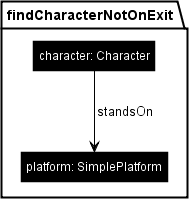
\includegraphics[scale=0.7]{../common/figures/pattern-findCharacterNotOnExit}
	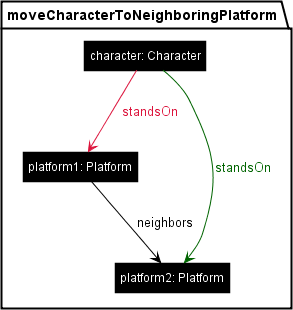
\includegraphics[scale=0.7]{../common/figures/rule-moveCharacterToNeighboringPlatform}
	\caption{Common Nodes of the Pattern \texttt{findCharacterNotOnExit} and the Rule \texttt{moveCharacterToNeighboringPlatform}}
	\label{fig:node-binding-common-nodes}
\end{figure}

\subsection{Parameters}
\label{api-parameters}
Patterns and rules may define parameters of primitive data types to be used in attribute assignments or conditions.
In contrast to node bindings, parameters are required.
When calling a pattern or rule, all parameters must be set in the constructor.
The parameter values may be changed using the setters.

Attribute conditions with parameters are filtered by the graph transformation interpreter similar to node bindings while all  other attribute conditions are checked by the pattern matching engine.
Parameterized attribute assignments will set the value of the parameter as new attribute value.
An example for this is shown in Listing~\ref{listing:parameters}:
The parameter for the color is passed to the pattern \texttt{findCharacterOfColor} (Figure~\ref{fig:pattern-findCharacterOfColor}) in the constructor (so it cannot be omitted!).
Without the parameter, the attribute condition could not be evaluated.
The interpreter knows all matches for the pattern reported by Democles and filters those for the ones whose color attribute has the given value \texttt{BLUE}.

\begin{lstlisting}[caption={Parameters}, label={listing:parameters}]
public void outputBlueCharacters() {
	api.findCharacterOfColor(COLOR.BLUE)
		.forEachMatch(m -> {
			System.out.println(m.getCharacter().getName());
		});
}
\end{lstlisting}

\section{Exploiting the Incrementality}
\label{incrementality}
As eMoflon::IBeX-GT is based on an incremental pattern matcher, the incrementality can be exploited to support certain scenarios which are more difficult to implement without support for incrementality.
The following sections describe tasks which could not be easily supported without incrementality because they require permanent observation of all matches.
The incremental features add support for reactive programming \cite{SurveyReactiveProgramming}, which is based on automatic propagation of changes.

\subsection{Notification System}
\label{notification-system}
The pattern matcher permanently maintains a set of matches for all patterns and notifies the interpreter every time a new match appears or an existing match disappears.
This can be used to provide a notification system in the API: Subscribers can register themselves for notifications of appearing and disappearing matches.
If subscribers are registered, the interpreter forwards the notification of appearing or disappearing matches to them.

One application scenario is the permanent checking of constraints via reception of notifications whenever matches for the observed pattern appear or disappear.
For positive constraints there must be a match, otherwise the constraint is violated.
For negative constraints any reported match is a violation of the constraint.

In the context of the She Remembered Caterpillars game the notification system could be used to check whether the goal of the game (all characters stand on an exit platform) is reached by subscribing all matches for a character not on an exit platform:
As soon as the number of characters which are not on an exit platform reaches 0, the game is over.
Note that one needs to subscribe to the disappearing matches as well such that characters leaving an exit platform are added to the set again.
Listing~\ref{listing:notifications} shows the necessary code for initializing and maintaining the set of characters which have not reached their final destination yet.
The defined \texttt{Consumer}s will be called automatically whenever a change in the set of matches for the subscribed pattern is reported.

Without the notification system, one would need to check the subscribed pattern after every change in the model to be sure to notice that the game is over as soon as the last character reached an exit platform.
The incremental pattern matcher notices even changes made by third party-applications and not via the API -- and the changes in the set of matches triggers notifications if a subscription has been registered for those.

\begin{lstlisting}[caption={Subscription of Notifications}, label={listing:notifications}]
Set<Character> characters = new HashSet<Character>();

public void registerSubscriptions() {
	FindCharacterNotOnExitPattern notOnExit = api.findCharacterNotOnExit();
	notOnExit.matchStream()
		.map(m -> m.getCharacter())
		.forEach(c -> this.characters.add(c));
	notOnExit.subscribeDisappearing(m -> {
		this.characters.remove(m.getCharacter());
		checkEndOfGame();
	});
	notOnExit.subscribeAppearing(m -> {
		this.characters.add(m.getCharacter());
		checkEndOfGame();
	});
}

private void checkEndOfGame() {
	if (this.characters.size() == 0) {
		System.out.println("GAME OVER!");
	}
}
\end{lstlisting}

\subsection{Instant Automatic Rule Application}
\label{instant-automatic-rule-application}
Due to the notification of appearing matches, instant and automatic rule application can be easily supported.
If automatic rule application is enabled, the notification system will send a notification and the interpreter will apply the rule immediately after the new match appeared.
Note that this only holds for matches reported after enabling automatic rule applications.
Rule applications can be subscribed via the API's notification system.

Listing~\ref{listing:instant-application} shows an example of enabling automatic rule application.
Assuming that the rule \texttt{transformBlueAndRedToPurpleCharacter} (Figure~\ref{fig:rule-transformBlueAndRedToPurpleCharacter}) shall be applied as soon as a match for this rule is found, \ie a blue and a red character stand on the same platform.
Via a subscription of the rule applications, a \texttt{Consumer} outputs ``Automatic transformation'' on the console whenever the rule is applied.

\begin{lstlisting}[caption={Instant Automatic Rule Application}, label={listing:instant-application}]
public void enableAutoTransformations() {
	TransformBlueAndRedToPurpleCharacterRule transformation = api.transformBlueAndRedToPurpleCharacter();
	transformation.subscribeRuleApplications(m -> 
		System.out.println("Automatic transformation"));
	transformation.enableAutoApply();
}
\end{lstlisting}

\begin{figure}[h!]
	\centering
	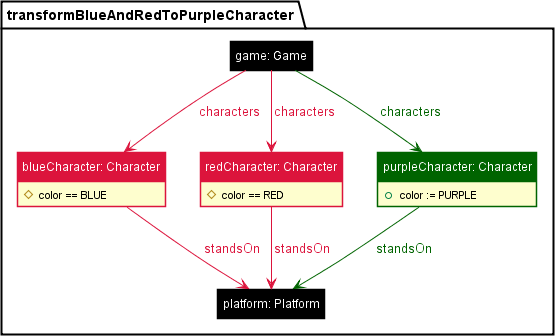
\includegraphics[scale=0.7]{../common/figures/rule-transformBlueAndRedToPurpleCharacter}
	\caption{Rule \texttt{transformBlueAndRedToPurpleCharacter}}
	\label{fig:rule-transformBlueAndRedToPurpleCharacter}
\end{figure}
